\section{Available resources}
\subsection{Time schedule}
The assignment and team members were assigned January 20. The initial meeting with the customer took place January 24, where the assignment was presented and discussed. Oral presentation of the project will be performed March 19 and the final deadline for submission of the project is set to May 30. The deadline for new specification that would result in major changes to the software is set to March 21., due to time restrictions.

\subsubsection{Available hours}
Each sprint has a duration of two weeks, excluding the period from April 4. to April 21., when the entire group leaves for a school field trip to China.

Table~\ref{tab:availHours} lists the project's available hours and is based on that all team members spends twenty hours on the project every week.

To compensate for the days the team will miss because of the school field trip mentioned above, the team has decided to increase the amount of work hours from 20 hours to 25 hours as of sprint 2 to and including sprint 6.

\begin{table}[H]
\centering
\rowcolors{1}{darkgray}{lightgray}
\begin{tabular}{|l|l|l|l|}
\hline
\textbf{Sprint \#} & \textbf{Dates} & \textbf{Days} & \textbf{Hours}\\
Sprint 1& January 27. - February 07. & 10  & 240 \\
Sprint 2 & February 10. - Februar 21. &10  & 300 \\
Sprint 3 & Februar 24. - March 07. &10 & 300 \\
Sprint 4 & March 10. - March 21. &10  &300 \\
Sprint 5 & March 24. - April 04. &10&  300 \\
Sprint 6 & April 21. - May 02. &10  &300 \\
\textbf{Total}&& \textbf{60}&  \textbf{1740}\\\hline
\end{tabular}
\caption{Available hours}
\label{tab:availHours}
\end{table}

\subsection{Milestones}
\begin{table}[H]
\centering
\rowcolors{1}{darkgray}{lightgray}
\begin{tabular}{|l|l|l|}
\hline
\textbf{Milestone \#} & \textbf{Description} & \textbf{Deadlines}\\
Milestone 1& Project report - preliminary version & February 9. \\
Milestone 2 & Project report - mid-semester version & March 16.  \\
Milestone 3 & Peer evaluation & March 23.  \\
 Milestone 4 & Project report - final version & May 30.\\\hline
\end{tabular}
\caption{Milestones}
\end{table}

\subsection{Gantt diagram}

A gantt diagram \ref{fig:gantt} is a representation of all the work hours, milestones and deadlines that is involved in the project. 

\begin{figure}[H]
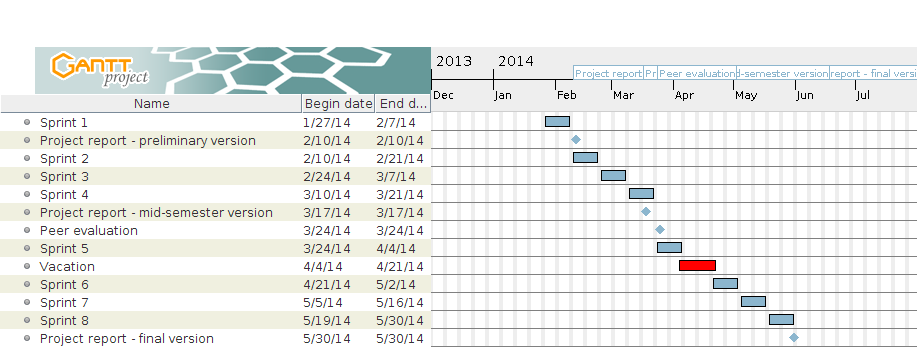
\includegraphics[width=\textwidth]{ch/projectPlan/fig/gantt.png}
\caption{The gantt diagram with sprints and milestones.}
\label{fig:gantt}
\end{figure}

\subsection{Supervisor from the Department of Computer and Information Science}
The team's supervisor is Alfredo Perez Fernandez. He is a PhD student at NTNU in the Department of Computer and Information Science~\cite{idi}. He may be contacted by e-mail at perezfer@idi.ntnu.no.

\subsection{Contact person at SINTEF}
The team's contact person at SINTEF is Babak Farshchian. He is an adjunct associate professor at NTNU and a researcher at SINTEF ICT~\cite{sintefict}. He may be contacted by e-mail at babak.farshchian@sintef.no.
